%Overskriftene er kokt rett fra prosess-rapport-presentasjonen. Endre dem.

\chapter{Oppstart og utvikling}

\section{Situasjon ved oppstart}

I første landsbydag fikk vi en kort introduksjon av konseptet bak landsbyen MiA.
Vi fikk informasjon om oppgaver som hadde blitt gjennomført tidligere. Blant
annet handlet en av oppgave om alpinski, og en annen om modellering av
matlaging. Samme dag fikk vi tildelt gruppe; Turid, Paul og Åsmund fra Fysikk og
matematikk, Joakim fra Bygg og miljøteknikk, og Knut Halvor fra Datateknikk. Vi
bestemte gruppas navn som ble Futhark. Resten av første landsbydag ble brukt
til å diskutere hvilket tema vi hadde lyst på. Det var litt klein stemning i
gruppa, men vi ble saktens kjent med hverandre. \\ 

\begin{figure}[ht!]
  \begin{center}
    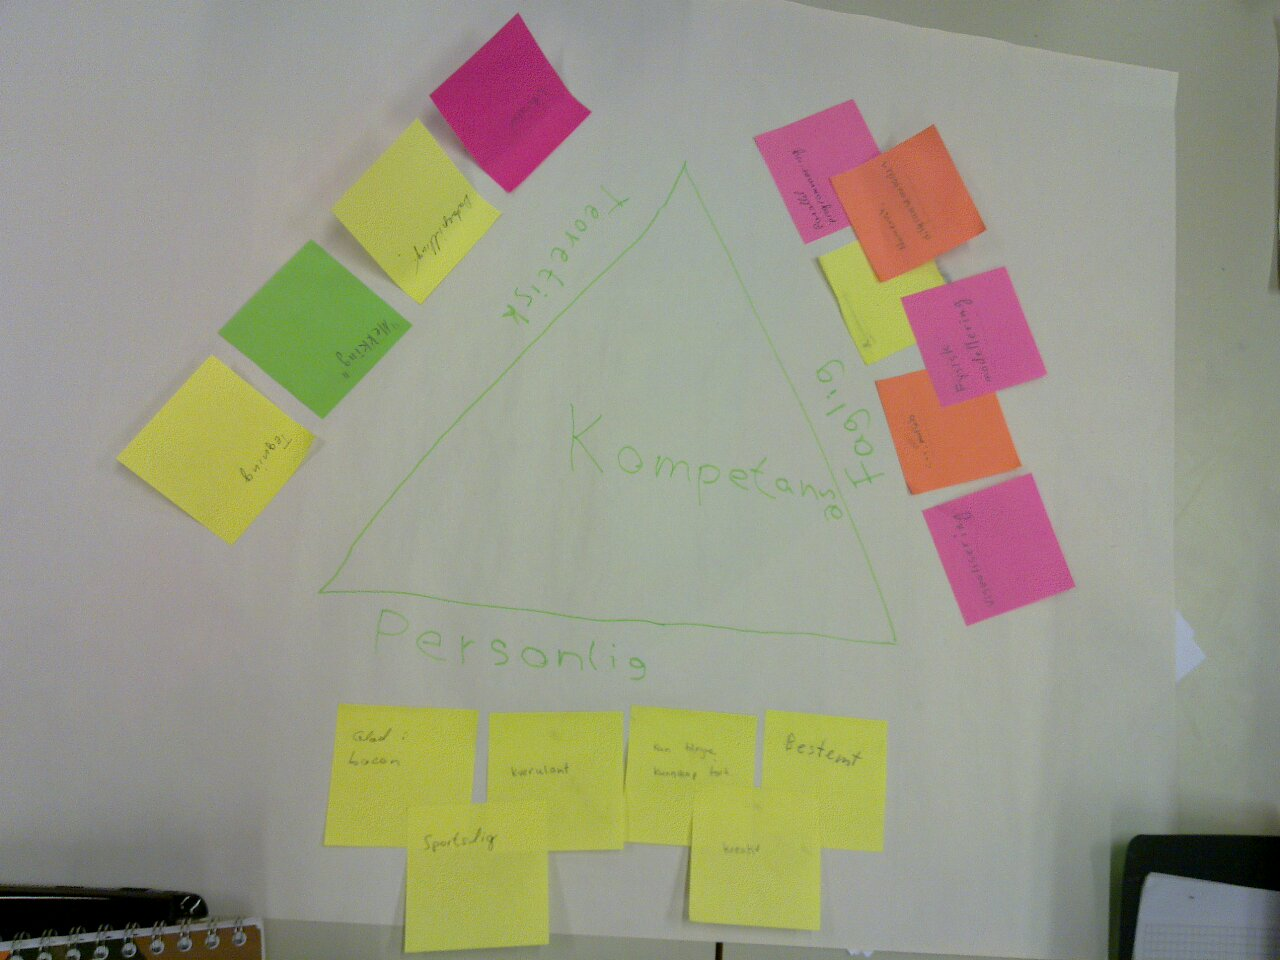
\includegraphics[width=0.8\textwidth]{kompetansetrekant.jpg}
  \end{center}
  \caption{Kompetansetrekant som gruppa lagde første landsbydag}
  \label{fig:kompetansetrekant}
\end{figure}

Andre landsbydag ble brukt til videre diskusjon av tema. Ved siden av hadde vi
en øvelse som gikk ut på å kartlegge kunnskapene til de enkelte gruppemedlemmene
i gruppa. Dette ble gjort ved at medlemmene førte sine kunnskapsområder på
en trekant med sider ”teoretisk”, ”faglige”, og ”personlige”,
\cref{fig:kompetansetrekant}. Med tanke på hva slags tema vi skulle velge, var
dette en god øvelse da
det var viktig å vite hva gruppa var i stand til gjøre. Etter en del diskusjoner
og løst prat hadde gruppa blitt bedre kjent, slik at folk torde å gi uttrykk for sine 
meninger.\\
 
I tredje landsbydag ble det iverksatt en øvelse som gikk ut på å presentere våre
erfaringer med gruppearbeid. Øvelsen var nyttig ettersom det gjorde det klart
hva slags roller gruppemedlemmene foretrakk å ha i et gruppearbeid. Samtidig ble
gruppa bedre kjent med hverandres arbeidsvaner. Samme dag fikk gruppa i oppgave
å tilegne seg teorien til Schwarz grupperegler \cref{sec:schwarz}. Teorien ble
tilegnet ved at hvert enkelt gruppemedlem skulle presentere sin del. Av
Schwarz’ grupperegler var de viktigste, etter vår mening, de to første: at
man tester sine antakelser og at man deler all relevant informasjon.  Vi fikk
erfare at når man ignorer disse reglene får det konsekvenser for
gruppedynamikken mye raskere enn vi hadde trodd. \\

Turid sa at hennes beste erfaring med gruppearbeid var fra håndball, noe Joakim
lo av. Det ble litt dårlig stemning, men diskusjonen ble hysjet ned av
fasilitatorene siden vi skulle gjøre individuelle oppgaver. Så emnet lå og
murret under overflaten til vi fikk snakke fritt igjen, da ble konflikten løst;
Turid sluttet av Joakims latter at det var hånlig ment, men det ble avklart at
Joakim ikke mente noe vondt med latteren.\\
%Reflekter mer!

Fra dette eksempelet kan man se at konflikten oppstod på grunn av
feiltolkninger; man hadde ikke kartlagt intensjonene bak det oppfattede
budskapet. Dette ble løst gjennom åpen diskusjon og deling av sine intensjoner
bak handlingene.  Etter de første landsbydagene hadde gruppa blitt godt kjent
med hverandre. Det var klart hva de enkelte gruppemedlemmene var gode på, og
hvilke roller hver enkelte sannsynligvis ville ha i gruppesammenheng. Dermed var
alt tilrettelagt for gruppa til å velge oppgavetema.\\

\section{Formulering av problemstillingen}
Til å begynne med vurderte gruppa ``ski'' som tema for oppgaven. Ettersom Åsmund
stod mye på ski var dette en oppgave som interesserte ham veldig. De andre i
gruppa som ikke hadde så mye kunnskap om dette temaet var litt mer usikre. Det
ble diskutert hvilke problemer som kunne oppstå hvis vi valgte dette
som tema. Særlig Turid var kritisk, og det ble klart at det var flere
strukturelle utfordringer knyttet til denne oppgaven. De fleste i gruppa var
skeptiske fordi oppgaven virket komplisert og uklart definert. Gruppa kom til
slutt fram til at det var mange potensielle problemer som kunne oppstå hvis vi
valgte denne oppgaven.\\

Her blir det satt spørsmål ved gjennomførbarheten til fremlagte problemstilling. Dette
fører til en diskusjon rundt tema, der medlemmer legger frem fakta og mulige komplikasjoner 
som kan oppstå i arbeidet rundt oppgaven. Medlemmene legger også frem sine
synspunkt om hvorfor de er for eller imot temaet ski. Når avgjørelsen blir tatt
om å velge en ny problemstilling, sitter dermed alle medlemmer med all relevant informasjon så vel som interessene 
til de andre medlemmene i prosjektet. Vi følger her retningslinjene 2 og 5 i
Schwarz (\cref{tab:grunnregler})
regler for effektive grupper. Dette gjør at vi kan ta ein riktig avgjørelse,
basert på all fakta. Det er også 
viktig å notere seg at det fortsatt var muligheter for å velge denne problemstillingen, men 
det var i gruppas fellesinteresse å utforske andre muligheter. \\

Ny oppgave som ble foreslått skulle ha noe med mat å gjøre, da dette var et av
de tre hovedtemaene som ble presentert på første landsbydag. Etter lang
diskusjon om mulige matvarer ble bacon nevnt som et alternativ. Dette var det
stor begeistring for, og gruppa samlet seg raskt bak denne problemstillingen.
Gruppa var videre interessert i å inkludere flest mulig fagområder, samt å
gjøre noe som ikke lignet så mye på tidligere oppgaver. Mikrobølgeovn ble derfor
foreslått som stekemedium fordi det inkluderte både numeriske og fysiske
problemer. Oppgaven inkluderte også visualisering av resultatet, noe som passet for Knut
Halvor siden han har drevet med det tidligere. Derfor endte det hele
med at vi valgte dette som tema i prosjektet.\\

Etter en lengre og åpen diskusjon klarte vi altså å komme frem til en problemstilling 
alle var fornøyde med og følte eierskap til. Dette var et viktig mål for gruppen, 
da resultatet for prosjektdelen, såvel som prosessdelen - i stor 
grad avhenger av dette. Vi har også hatt fokus på å prøve og innlemme alle
medlemmers individuelle kompetanse i problemstillingen. Med unntak av Joakim,
følte vi at vi fikk til dette ganske bra.
Det var imidlertid en praktisk del i problemstillingen (eksperiment), som vi følte Joakim ville være bra egnet 
til å ha ansvar for, på grunn av hans kompetanse som praktisk anlagt.
I etterkant ser vi at dette har fungert bra,
hvert medlem har fått et eget ansvarområde på prosjektet, noe som ga naturlig
eierskap til prosjektet. Dette er i god overenstemmelse med J\&Js gruppeteori,
se \cref{sec:jj}.\\

%Videre ble det anskaffet en del litteratur slik at vi kunne finne ut hva vi
%kunne gjøre. Vi fant ut at det fantes en del publikasjoner rundt dette temaet.
%Mye tid ble derfor brukt til å finne litteratur til å gi oss en idè om hvordan
%vi skulle gå løs på oppgaven. For å lette på samarbeidet mellom gruppemedlemmene
%ble det satt opp en konto slik at vi kunne dele kode og annet informasjon via
%internettet.\\

%I fjerde landsbydag fikk gruppa i oppgave å presentere oppgaven vi hadde valgt,
%og litt hvordan vi skulle løse den. Dette medførte til at gruppa ble mer
%fokusert på hva vi skulle gjøre. Ettersom det begynte å bli en del arbeid,
%gjorde Turid en aksjon og delte ut oppgaver til gruppemedlemmene. 
%Dette gjorde hun fordi hun var frustrert over manglende initiativ. Gruppa opplevde da
%at Turid hadde en styrende rolle i gruppa. Likevel mente gruppa at dette var positivt
%fordi det var nødvendig å få til aksjoner for at gruppas mål skulle bli nådd. Ifølge teorien
%presentert i \cref{avs:roller} hadde Turid en rolle som oppgaveleder. 
%
%\section{Opprinnelig plan}
%Gruppas opprinnelige plan var å løse varmelikningene og transportlikningen for
%bacon. Når dette var avgjort trengtes en mer detaljert plan. Den første
%diskusjonen som oppstod var om vi skulle bruke en eksplisitt eller implisitt
%numerisk metode. Knut, som har hovedansvaret for implementasjon, ville gjerne
%bruke en metode som enkelt kunne implementeres. Matematikerne ville
%på den andre siden bruke en mer avansert modell, som var vanskeligere å ta i
%bruk. Dette ble diskutert over en lengre periode, med innspill fra landsbyleder
%om at det var bedre å satse på et ambisiøst prosjekt. Til slutt ble også Knut
%overbevist om å bruke en implisitt metode, slik at de ble konsensus i gruppa. I
%ettertid ser vi at dette medførte en mye større arbeidsoppgave for Knut, men han
%har gått løs på oppgaven med godt mot. 
%
%Når denne hindringen var overkommet satte vi ned en liste med prioriterte mål
%som skulle oppnås, og noen mål som kunne vurderes dersom de første var
%nådd. Prioriteringen av mål var det liten splid rundt, og hele denne prosessen
%gikk nokså effektivt, delvis fordi medlemmene var innstilte på å ha en plan slik
%det står i samarbeidskontrakten. 
%Refleksjon! Jamfør teori om at grupper trenger konkrete mål.
%De siste alternative punktene var morsomme selv om de var ambisiøse =>
%inspirerer gruppa til å arbeide.

\section{Regler, avtaler, kontrakt}
\label{sec:kontrakt}
Nødvendigheten av å ha klare regler og avtaler innad i en gruppe diskuteres i
mange av pensumartiklene. I Schwarz' ``Ground rules for Effective Groups''
\cite{schwarz} nevnes det som ett av ni punkter avgjørende for en effektiv
gruppe: ``Etabler regler for hvordan avgjørerelser
tas''. Johnson \& Johnson påpeker i ``Valuing Diversity'' \cite{jj} hvor viktig det er at gruppa skaper seg en felles
identitet, som hvert gruppemedlem kan samles bak. En samarbeidskontrakt, med
regler for håndtering av konflikter, hvordan avgjørelser tas, straff for
regelbrudd etc., fungerer nettopp på dette viset -
samlende. \\

Andre landsbydag var det satt av tid til å skrive samarbeidskontrakt. 
I \cref{avs:kontrakt} vises den reviderte kontrakten, med endringer fra den
originale uthevet. Det ble, i
samsvar med læringsassistentene, satt opp punkter for hvordan gruppa skulle
håndtere konflikter, ta avgjørelser og ikke minst - mål for gruppearbeid og
tidsfrister. Etter noen uker ble kontrakten reforhandlet. Det viste seg at
enkelte punkter var redundante, mens andre måtte legges til. Særs punktet om
kaffemøtene før oppstart har vist seg effektivt, da det tilbyr en uhøytidelig
setting hvor synspunkter kan deles og diskuteres. Det ble i
tillegg lagt merke til at gruppemedlemmenes individuelle oversikt var manglende, og et nytt
punkt vedrørende fremdriftsplaner ble lagt til. Noe som ble fjernet var punktet
om at alle oppgaver skulle føres inn på gruppas wiki-side, da det \textbf{1)} aldri ble
fulgt opp, og \textbf{2)} til en viss grad ble erstattet med det nye punktet om
fremdriftsplan. \\

Gruppa hadde lagt merke til at punktet om tildelte oppgaver skulle føres
inn på wiki-siden aldri ble brukt. At kun tre på gruppa (Joakim, Åsmund og Knut)
hadde kjennskap til github (stedet hvor gruppa lagrer informasjon) kan til dels
ta skylden for det. I tillegg påvirket mangelen av en fremdriftsplan hvert
gruppemedlems oppfatning av egne arbeidsoppgaver. Etter som tiden gikk ble det
endel murring fra Paul og Turid, som følte at det var vanskelig
å følge utviklingen. Det ble derfor avtalt at gruppa skulle møtes førstkommende
søndag, slik at samtlige gruppemedlemmer skulle få en innføring i, samt lære seg
bruken av github. \\

Bruken av github har imidlertid ikke bare hatt negative konsekvenser, det har blant annet
ført til at føring av timer utenfor avsatt kjernetid har skjedd automatisk. Et
plott av tidsbruk for hele gruppa vises i \cref{fig:punchcard}, der abcissen
viser klokkeslett og ordinaten viser ukedager.
\begin{figure}[H]
  \begin{center}
    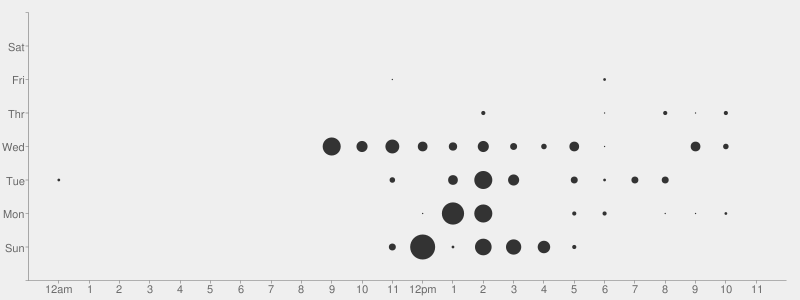
\includegraphics[width=\textwidth]{punchcard.png}
  \end{center}
  \caption{Punchcard som viser antall endringer på github vom funksjon av tid}
  \label{fig:punchcard}
\end{figure}
%Tving denne figuren til å oppføre seg - done, Åsmund
Fra denne figuren framgår det at onsdag og søndag hovedsaklig har vært gruppas
jobbedager, der gruppa har møttes og arbeidet sammen. I tillegg har det blitt satt
frister til onsdag for at ting skal være gjort, noe som reflekteres i at mye
arbeid har skjedd på mandag og tirsdag. Til sammenlikning er torsdag, fredag og
lørdag nesten uten arbeid.\\

\section{Beslutningsmønstre}
I gruppekontrakten (se \cref{avs:kontrakt}) står det at beslutninger fortrinnsvis
skal tas basert på konsensus, mens det ved splid skal være flertallsavgjørelse.
Gruppa var tidlig innstilt på konsensusavgjørelser, da det sørger for gode og
grundige diskusjoner ved uenighet, og kan i den forstand virke veldig samlende
for en gruppe. Likevel innså vi at enkelte situasjoner kunne bli fullstendig
fastlåst, slik at flertallet måtte få bestemme. Det er likevel viktig at
konsensus har blitt \emph{forsøkt} oppnådd før flertallsavgjørelse
implementeres. \\

Den første avgjørelsen gruppa tok var valg av oppgave. Åsmund var i starten
veldig giret på skiforsøket, som gikk ut på å måle spenstforfallet i en
slalomski utover sesongen. Resten av gruppa var noe mer moderate i
begeistringen. Det ble derfor arrangert ``høring'' hvor samtlige gruppemedlemmer
kom med forslag. Disse ble så samlet og diskutert, og gruppa forsøkte å finne en
oppgave hvor alle kunne bidra. Valget falt derfor på steking av bacon i
microbølgeovn, da dette hadde et massivt innslag av numerikk, programmering og
fysikk. Disipliner gruppa dekte meget godt mellom seg. \\

I samarbeidskontrakten er gruppestrukturen betegnet som ``riddere av det runde
bord''. Dette er et prinsipp som anvendes i alle våre beslutninger. Når et
problem oppstår går ordet rundt bordet, og hvert gruppemedlem sier sin mening.
Det diskuteres deretter i plenum, og om mulig oppnås en konsensusavgjørelse. Vi
har kun ved ett tilfelle anvendt flertall-paragrafen i kontrakten og det var i
forbindelse med språkvalg på prosessrapporten. Knut var i utgangspunktet uvillig
til å skrive på norsk, og det gikk ikke å ``vinne'' han over. Etter en god stund
med diskusjon ble altså Knut Halvor overstyrt.\\

\section{Roller i gruppa}
\begin{quote}
``En person blir en leder når han eller hun blir satt i en lederposisjon.''
\end{quote}

I gruppekontrakten ble det bestemt at vi skulle ha en flat struktur i gruppa. Valget 
var basert på at ingen egentlig ville gå inn i en lederrolle, og at vi ville ha en 
større frihet til å formulere arbeidsoppgavene selv. Vi kom likevel opp i situasjoner
som krevde at en person tok ledelse for å sikre effektiviteten til gruppa. I praksis 
fikk gruppa en situasjonsbetinget lederstruktur. Situasjonsbetinget lederskap er definert
som delt lederskap blant gruppemedlemmer der medlemmene varierer oppførselen etter hva
funksjon gruppa trenger til enhver tid, der en funksjon er en aksjon som blir satt 
igang for å sikre effektiviteten i gruppa.\\

Den situasjonsbetingede lederstrukturen førte til at gruppemedlemmer tok rollen som 
leder i den fagdelen de hadde mest autoritet på. Åsmund ble dermed en uformell leder 
for fysikkdelen, Turid for numerikkdelen og Knut for programmeringsdelen. De 
tok dermed ansvar for fremgangen og oppgavedeling på disse områdene, og strukturerte
samarbeidet mellom gruppemedlemmene på sitt respektive felt. \\

I vår gruppe så vi at Åsmund i større grad gikk inn i rollen som oppgave-leder. Han 
tok ansvar for å sette opp et system for utveksling av informasjon rundt prosjektet, 
github, og tok ofte initiativ ved å legge ut relevante artikler på siden. Han gikk 
dermed inn i rollen som koordinator \cref{avs:roller} på gruppa. Vi merket oss og at han var 
mer aktiv i prosjektet i EIT, som er den delen som er mest oppgavefokusert. \\

Bales statuerer at medlemmer som er veldig oppgavefokusert er mindre involvert i 
relasjonsrettede aksjoner. Paul er den i gruppa som er mest oppgavefokusert. 
På gruppa har han en tendens til å ta en faglig tilnærming, og liker å fokusere mest 
på oppgaven for hånd. Han faller altså oftere inn i rollen som diagnostiker og 
informasjonssøkeren, se \cref{avs:roller} for en definisjon av rollene. Paul er dermed en styrke på gruppa ved at han holder 
diskusjonene relevante, i tillegg til at han er et pålitelig medlem når det gjelder 
å gjennomføre arbeidet i tide. Vi ser likevel en tendens til at Paul er mindre involvert 
i relasjonsrettede aksjoner på gruppa. 
Den som oftest gikk inn i rollen som sosial-emosjonell leder var Turid. Hun var et viktig 
ledd i gruppa i form av å uttrykke klare meninger og frustrasjon over sider ved gruppa
som ikke fungerte optimalt. Hun gikk dermed inn i rollen som kritiker og følelsetolker.
Når det var ting som fungerte bra i gruppa kom hun inn med støtte og oppmuntring til å 
fortsette på samme linje. Selv om hun var en av de som oftest var involvert i diskusjoner/konflikter,
var hun og ofte den som løste de, enten gjennom forhandlinger eller ved å trekke seg tilbake
når hun gikk for langt. Turid var og det medlemmet i gruppa som oftest tok initiativ og ledelse 
i prosessdelen av EiT, som fokuserer mest på relasjoner og samarbeid mellom medlemmer på gruppa. 
Her virket hun ofte som målvakt, ved å igangsette runde rundt bordet og være oppmerksom på 
at alle kom til ordet. Vi legger merke til at de situasjonene der Turid har
lederrollen i gruppa gjør at hennes rolle implisitt ligner mer på en tradisjonelle lederrolle, der de
andre har mer fagspesifikke lederroller. \\

Bales statuerer og at sosial-emosjonelle aksjoner ofte blir igangsatt av medlemmer som er 
mindre involverte i oppgaveretta aksjoner. Dette ser vi igjen i gruppa ved at Joakim var 
involvert flere sosial-emosjonelle aksjoner. Denne situasjonen har oppstått ved at prosjektet 
er noe utenfor hans fagfelt, og han er dermed blitt mindre involvert i selve oppgaveløsingen. 
Joakim har delvis valgt dette bevisst ved en landsby der hans fagkompetanse ikke
står sterkest. Da hans rolle blir mindre faglig, kommer han naturlig inn i en
rolle som er mer i retning av en fasilitator for godt gruppemiljø. At ett av
gruppemedlemmene har hatt en slik rolle, i tillegg til å bidra faglig, har
utvilsomt gjort at gruppa har hatt høy ytelse når vi jobber, og heller tar
naturlige pauser med god stemning og humor når medlemmene er slitne. Dette har
nok også hatt en effekt på at medlemmene i gruppa ble fort kjent med hverandre.
Joakim har utfylt denne rollen blant annet ved å alltid stille med en positiv innstilling og 
å involvere gruppa i diskusjoner som går på andre ting enn kun det faglige.\\

Det bor en liten kritiker i samtlige medlemmer på gruppa. Vi ser likevel at Knut har tatt på 
seg denne rollen i gruppa i større grad enn andre. Kritikeren er viktig i gruppesammenheng 
ved «systematisk, åpen, støttende og kritisk gransking av sitt og andres bidrag til gruppearbeidet.»
Dette gjøres på en slik måte at medlemmer på gruppa ikke opplever kritikken som en trussel, 
og dermed beholder fokuset på oppgaveløsning. Knut tar også på seg rollen som meningssøkeren, 
ved at han oppfordrer til at gruppemedlemmene skal få sagt sin mening slik at en beslutning
kan tas.\\

\begin{figure}[H]
\centering
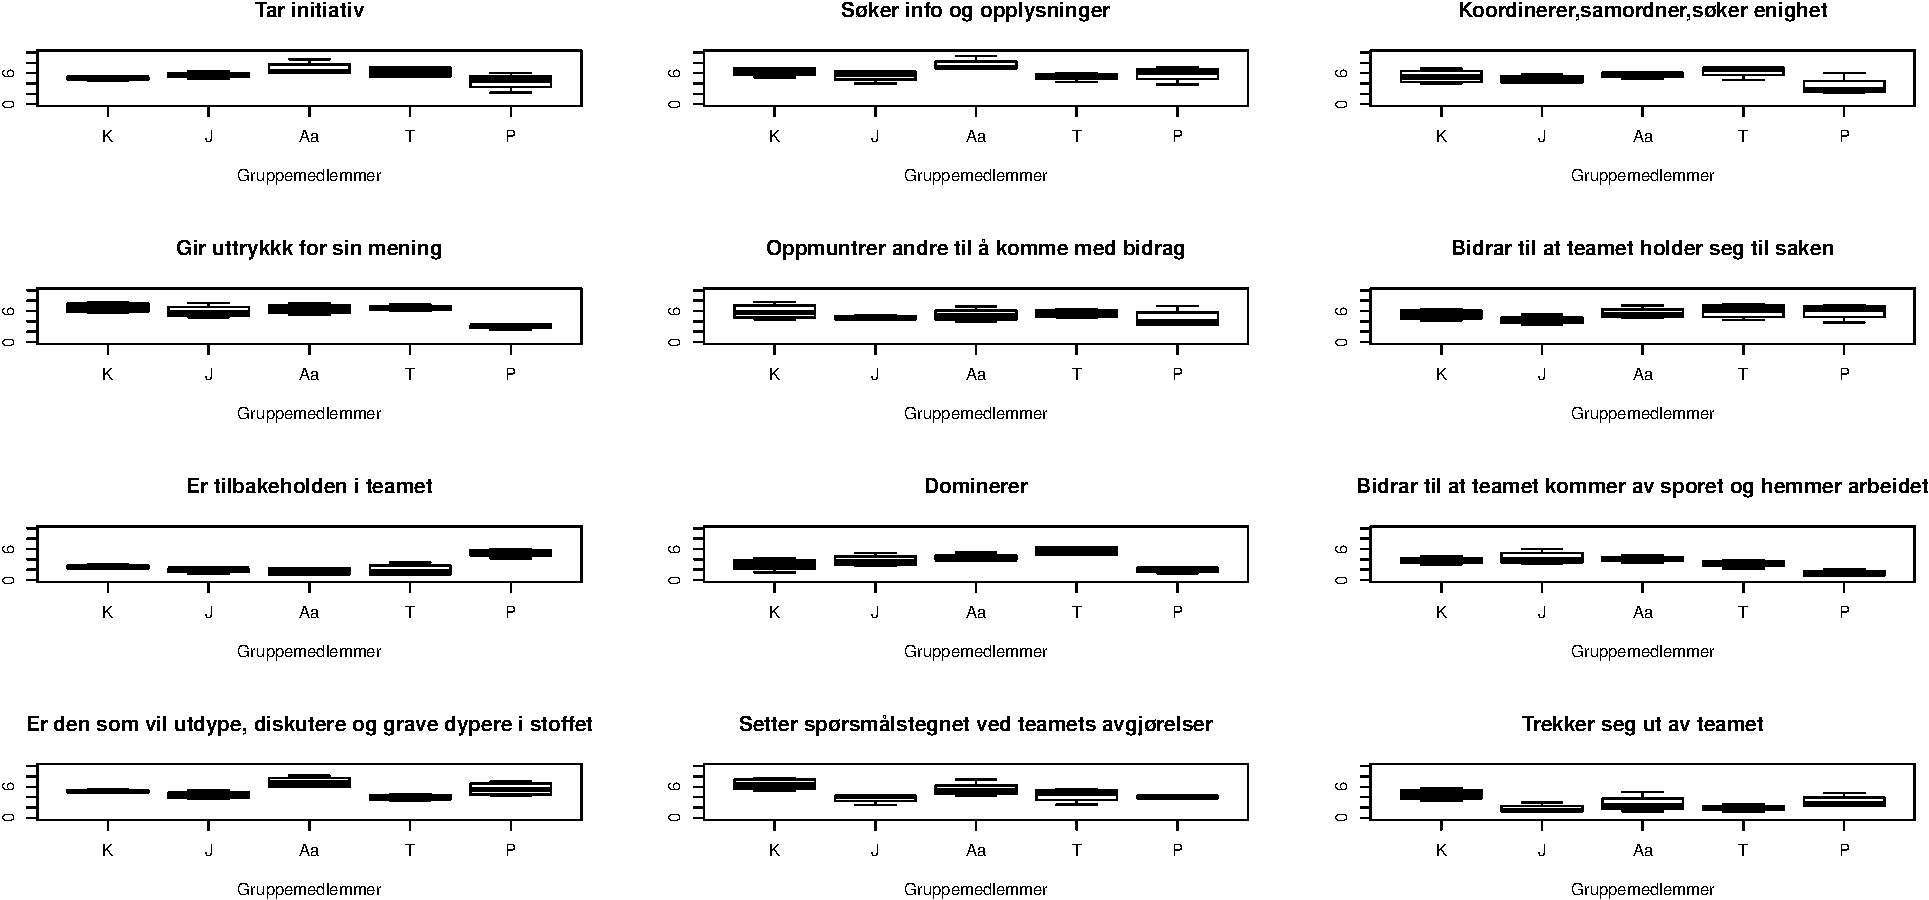
\includegraphics[scale=0.4]{teammedlem.pdf}
\caption{Plot av egenskaper til medlemmer på gruppa}
\label{fig:medlemmer}
\end{figure}

I \cref{fig:medlemmer} har vi brukt den ene prosessøvelsen til å
lage et plot over egenskapene til gruppemedlemmene. Vi ser at de personlige
 egenskapene er reflektert i de rollene gruppemedlemmene har påtatt seg i gruppa. Som gruppas
kritiker ser vi at Knut skårer høyt, han setter ofte spørsmålstegn ved teamets avgjørelser. 
Han skårer også høyere på punktet ``trekker seg ut av teamet'', som igjen kan trekkes tilbake 
til at han har en lederposisjon ved implementering av
programmet. Joakim skiller seg mest fra gruppa på punktet ``Bidrar til at teamet 
sporer av''. Det kan relateres tilbake til Joakims rolle som energigiver. Den beste måten å lade opp igjen
for videre jobbing med prosjektet er ofte ved å få litt adspredelse fra selve oppgavejobbinga.
Åsmund skårer høyt på punkta ``tar initiativ'' og ``søker info og opplysninger''. 
Dette kan relateres til lederrollen Åsmund har tatt for fysikkdelen av prosjektet,
som er veldig teoretisk. (Når en prøver å modellere en prosess realistisk kan
modellen raskt bli komplisert. Det er da viktig at vi har nok informasjon til å
kunne gjøre forenklinger som fremdeles resulterer i et realistisk modell).
Turid er den som skårer høyest på punktet ``dominerer og koordinerer, samordner, søker
enighet'', som igjen kan relateres tilbake til den rollen hun har hatt som
sosial-emosjonell leder. Ellers legger vi merke til at gruppa
generelt er flinke til å ta initiativ, søke info/opplysninger og gi uttrykk for sine meninger. Paul
er den i teamet som er mest oppgavefokusert, og vi ser en tendens i modellen til
at han skårer noe høyere på ``tilbakeholden i teamet''.\\

\section{Tilbakeblikk}
\label{sec:tilbakeblikk}

Når vi ser tilbake kan det påstås at gruppa gjennomgikk de fire trinnene i
Tuckmans \cite{tuckman} teori om gruppeutvikling, \emph{forming, storming,
norming} og \emph{performing}, kort oppsummert sier Tuckman at gruppen først vil
formes, en fase som kjennetegnes ved bred enighet og lite konflikt. Deretter
følger motstandsfasen (storming) hvor det stormer rundt medlemmene, det er
konflikter og problemer. Disse løses i norming-fasen, og gruppa blir enig om
hvordan konflikter og problemer skal løses. Gruppa blir da i stand til å
prestere i performing-fasen. Vi har lagt merke at gruppa tildels har hoppet helt over
\emph{storming}-fasen. Dette har sin årsak i at vi er rimelig like i måten å
håndtere konflikter og at vi ikke kverulerer unødvendig, men er heller
løsningsorienterte og har fokus på fremdrift. At Tuckmans modell ikke passer
helt i dagens grupper (det er en gammel teori fra 1965), passer godt med Endre
Sjøvolds \cite{sjovold} påstander om at den er i ferd med å bli overflødig. Vi
kjenner oss også godt igjen i Sjøvolds evaluering av EiT-grupper, som basert på
Systematisere Person-Gruppe Relasjonen-modellen (SPGR) sier at utviklingen i en
EiT-gruppe ikke er signifikant (se \cref{tab:sjovold}).\\

\begin{table}[H]
\centering
\begin{tabular}{l c c}
\toprule
& Pre & Post  \\
\midrule
Kontroll & 3.15 & 3.00 \\
Åpenhet & 4.71 & 4.61 \\
Avhengighet & 5.54 & 5.48 \\
Opposisjon & 1.50 & 1.36 \\
Innesluttethet & 1.20 & 1.09 \\
Synergi & 6.51 & 6.54 \\
\bottomrule
\end{tabular}
\caption{Resultater fra Sjøvolds studie av EiT-grupper over ett semester, ser at
det ikke er noen signifikant forandring før/etter.}
\label{tab:sjovold}
\end{table}

Vi har likevel en kommentar til Sjøvolds konklusjon vedrørende kategorien
\emph{åpenhet}. Selv om gruppas åpenhet er uendret, har kommunikasjonen blitt
tryggere og medlemmene trenger ikke ta like mye hensyn til mottakers følelser, 
slik at eksponeringen over tid har gjort interaksjonen mellom
medlemmene mer ukomplisert. Vi erkjenner også at rollene hver enkelt påtok
seg ved starten, har forblitt tilnærmet uforandret gjennom semesteret.

Vi la vi merke til den største endringen i gruppas samspill under framføringen i midten av
semesteret. Vi fikk følelsen av at de andre på gruppa var støttende og
oppmerksomme når vi presenterte, og hvis vi fikk problemer med noe var de andre
medlemmene støttende og kom med innspill. Dette førte også til at flere av
medlemmene improviserte med eksempler rundt prosessbiten og gruppas framgang,
fordi vi følte at tryggheten og støtten var der.

